
\subsection{Listas de adyacencia}
\label{sec:listas_de_adyacencia}

Otra forma de representar un grafo es mediante un arreglo de \(n = \abs{V}\) apuntadores. Cada apuntador representa un vértice \(v\) y apunta a una lista (simple o doblemente) encadenada, cuyos valores representan a los vértices que son sucesores de \(v\), en un grafo dirigido, o que son adyacentes a \(v\), en un grafo no dirigido.

\begin{definicion}{Lista de adyacencia}{lista_de_adyacencia}
  Sea \(G\) un grafo simple o dirigido, con vértices \(v_0, \ldots, v_{n-1}\), la \concept{lista de adyacencia} de \(G\) es un arreglo \(L\) de tamaño \(n\) tal que \(L[i]\) es la lista encadenada de valores \(j\) tales que \(v_i \longrightarrow v_j\).
\end{definicion}

Si \(G\) es además ponderado, cada nodo de la lista encadenada de \(L[i]\) almacena, junto con el vértice \(v_j\), el peso \(w(v_i, v_j)\) del arco correspondiente.

\begin{center}
  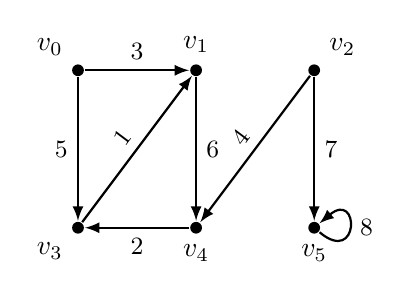
\begin{tikzpicture}[baseline=(current bounding box.center),
    vertex/.style={circle, fill=black, inner sep=1.5pt},
    -latex, thick,
  ]
    \node[vertex, label=above left:\(v_0\)]  (v0) at (0, 2)   {};
    \node[vertex, label=above:\(v_1\)]       (v1) at (1.5, 2) {};
    \node[vertex, label=above right:\(v_2\)] (v2) at (3, 2)   {};
    \node[vertex, label=below left:\(v_3\)]  (v3) at (0, 0)   {};
    \node[vertex, label=below:\(v_4\)]       (v4) at (1.5, 0) {};
    \node[vertex, label=below:\(v_5\)]       (v5) at (3, 0)   {};

    \draw (v0) -- (v1) node[midway, above] {\small 3};
    \draw (v0) -- (v3) node[midway, left] {\small 5};
    \draw (v3) -- (v1) node[midway, above, sloped] {\small 1};
    \draw (v1) -- (v4) node[midway, right] {\small 6};
    \draw (v4) -- (v3) node[midway, below] {\small 2};
    \draw (v2) -- (v4) node[midway, above, sloped] {\small 4};
    \draw (v2) -- (v5) node[midway, right] {\small 7};
    \draw (v5) to[out=-40, in=40, looseness=15] node[right] {\small 8} (v5);
  \end{tikzpicture}
  \hspace{1.5cm}
  \begin{tikzpicture}[baseline=(current bounding box.center),
    idxcell/.style={draw, minimum size=0.42cm, inner sep=0pt, outer sep=0pt},
    slot/.style={draw, minimum size=0.42cm, inner sep=1pt, outer sep=0pt, font=\scriptsize},
    -latex, thick,
  ]
    \node[idxcell]                    (idx0) at (0, 0) {};
    \node[idxcell, below=0pt of idx0] (idx1) {};
    \node[idxcell, below=0pt of idx1] (idx2) {};
    \node[idxcell, below=0pt of idx2] (idx3) {};
    \node[idxcell, below=0pt of idx3] (idx4) {};
    \node[idxcell, below=0pt of idx4] (idx5) {};

    % idx0: v1:3, v3:5
    \node[slot, right=0.35cm of idx0] (r0a1) {1};
    \node[slot, right=0pt of r0a1]    (r0a2) {3};
    \node[slot, right=0pt of r0a2]    (r0a3) {};
    \node[slot, right=0.35cm of r0a3] (r0b1) {3};
    \node[slot, right=0pt of r0b1]    (r0b2) {5};
    \node[slot, right=0pt of r0b2]    (r0b3) {};
    \draw (idx0.center) -- (r0a1);
    \draw (r0a3.center) -- (r0b1);

    % idx1: v4:6
    \node[slot, right=0.35cm of idx1] (r1a1) {4};
    \node[slot, right=0pt of r1a1]    (r1a2) {6};
    \node[slot, right=0pt of r1a2]    (r1a3) {};
    \draw (idx1.center) -- (r1a1);

    % idx2: v4:4, v5:7
    \node[slot, right=0.35cm of idx2] (r2a1) {4};
    \node[slot, right=0pt of r2a1]    (r2a2) {4};
    \node[slot, right=0pt of r2a2]    (r2a3) {};
    \node[slot, right=0.35cm of r2a3] (r2b1) {5};
    \node[slot, right=0pt of r2b1]    (r2b2) {7};
    \node[slot, right=0pt of r2b2]    (r2b3) {};
    \draw (idx2.center) -- (r2a1);
    \draw (r2a3.center) -- (r2b1);

    % idx3: v1:1
    \node[slot, right=0.35cm of idx3] (r3a1) {1};
    \node[slot, right=0pt of r3a1]    (r3a2) {1};
    \node[slot, right=0pt of r3a2]    (r3a3) {};
    \draw (idx3.center) -- (r3a1);

    % idx4: v3:2
    \node[slot, right=0.35cm of idx4] (r4a1) {3};
    \node[slot, right=0pt of r4a1]    (r4a2) {2};
    \node[slot, right=0pt of r4a2]    (r4a3) {};
    \draw (idx4.center) -- (r4a1);

    % idx5: v5:8
    \node[slot, right=0.35cm of idx5] (r5a1) {5};
    \node[slot, right=0pt of r5a1]    (r5a2) {8};
    \node[slot, right=0pt of r5a2]    (r5a3) {};
    \draw (idx5.center) -- (r5a1);
  \end{tikzpicture}
  \captionof{figure}{Un grafo dirigido, ponderado y disperso junto a sus listas de adyacencia.}
  \label{fig:lista_de_adyacencia}
\end{center}

\subsubsection{Complejidad espacial}

El costo en espacio de las listas de adyacencia radica en dos cosas: una son los \(n\) apuntadores, uno a cada lista; la segunda, son cuántos elementos hay en total en todas las listas.

Si el grafo es no dirigido, se representa cada arista dos veces: en la lista del primer nodo y en la lista del segundo, por lo que la cantidad de elementos es de \(2\varepsilon\). Si es dirigido, se almacena cada arista una vez, solo \(\varepsilon\) elementos.

En cualquier caso, la complejidad espacial es entonces \(\Theta(n+\varepsilon)\).

\subsubsection{Comparación}
\label{sec:comparacion}

La clara ventaja de las listas de adyacencia es el espacio que se ahorra respecto a la matriz de adyacencia al no representar la ausencia de arcos.

El pago por ese ahorro es que las operaciones que se realizan sobre una arista son lineales, \(\Theta(d)\) donde \(d\) es el grado de alguno de los vértices de la arista, en lugar de constantes.

Conocer el grado de un vértice es de costo constante si cada lista encadenada almacena su longitud como metadato, que es común en implementaciones de listas encadenadas.